\section{Das Semesterticket -- die neue Freiheit}

\begin{center}
	\includegraphics[width=\textwidth, height=0.2\textheight]{res/bus_und_bahn.pdf}
\end{center}
\begin{multicols*}{2}
\begin{figure*}[t]
	\subsection{NRW Regionalverkehrsplan}
	% XXX Jedes Jahr Regionalverkehrsplan aktualisieren
	% Quelle Regionalverkehrsplan:
	% https://www.vrr.de/de/fahrplan-mobilitaet/stadt-linien-netzplaene/
	% https://infoportal.mobil.nrw/information-service/regionalverkehrsplan-nrw.html
	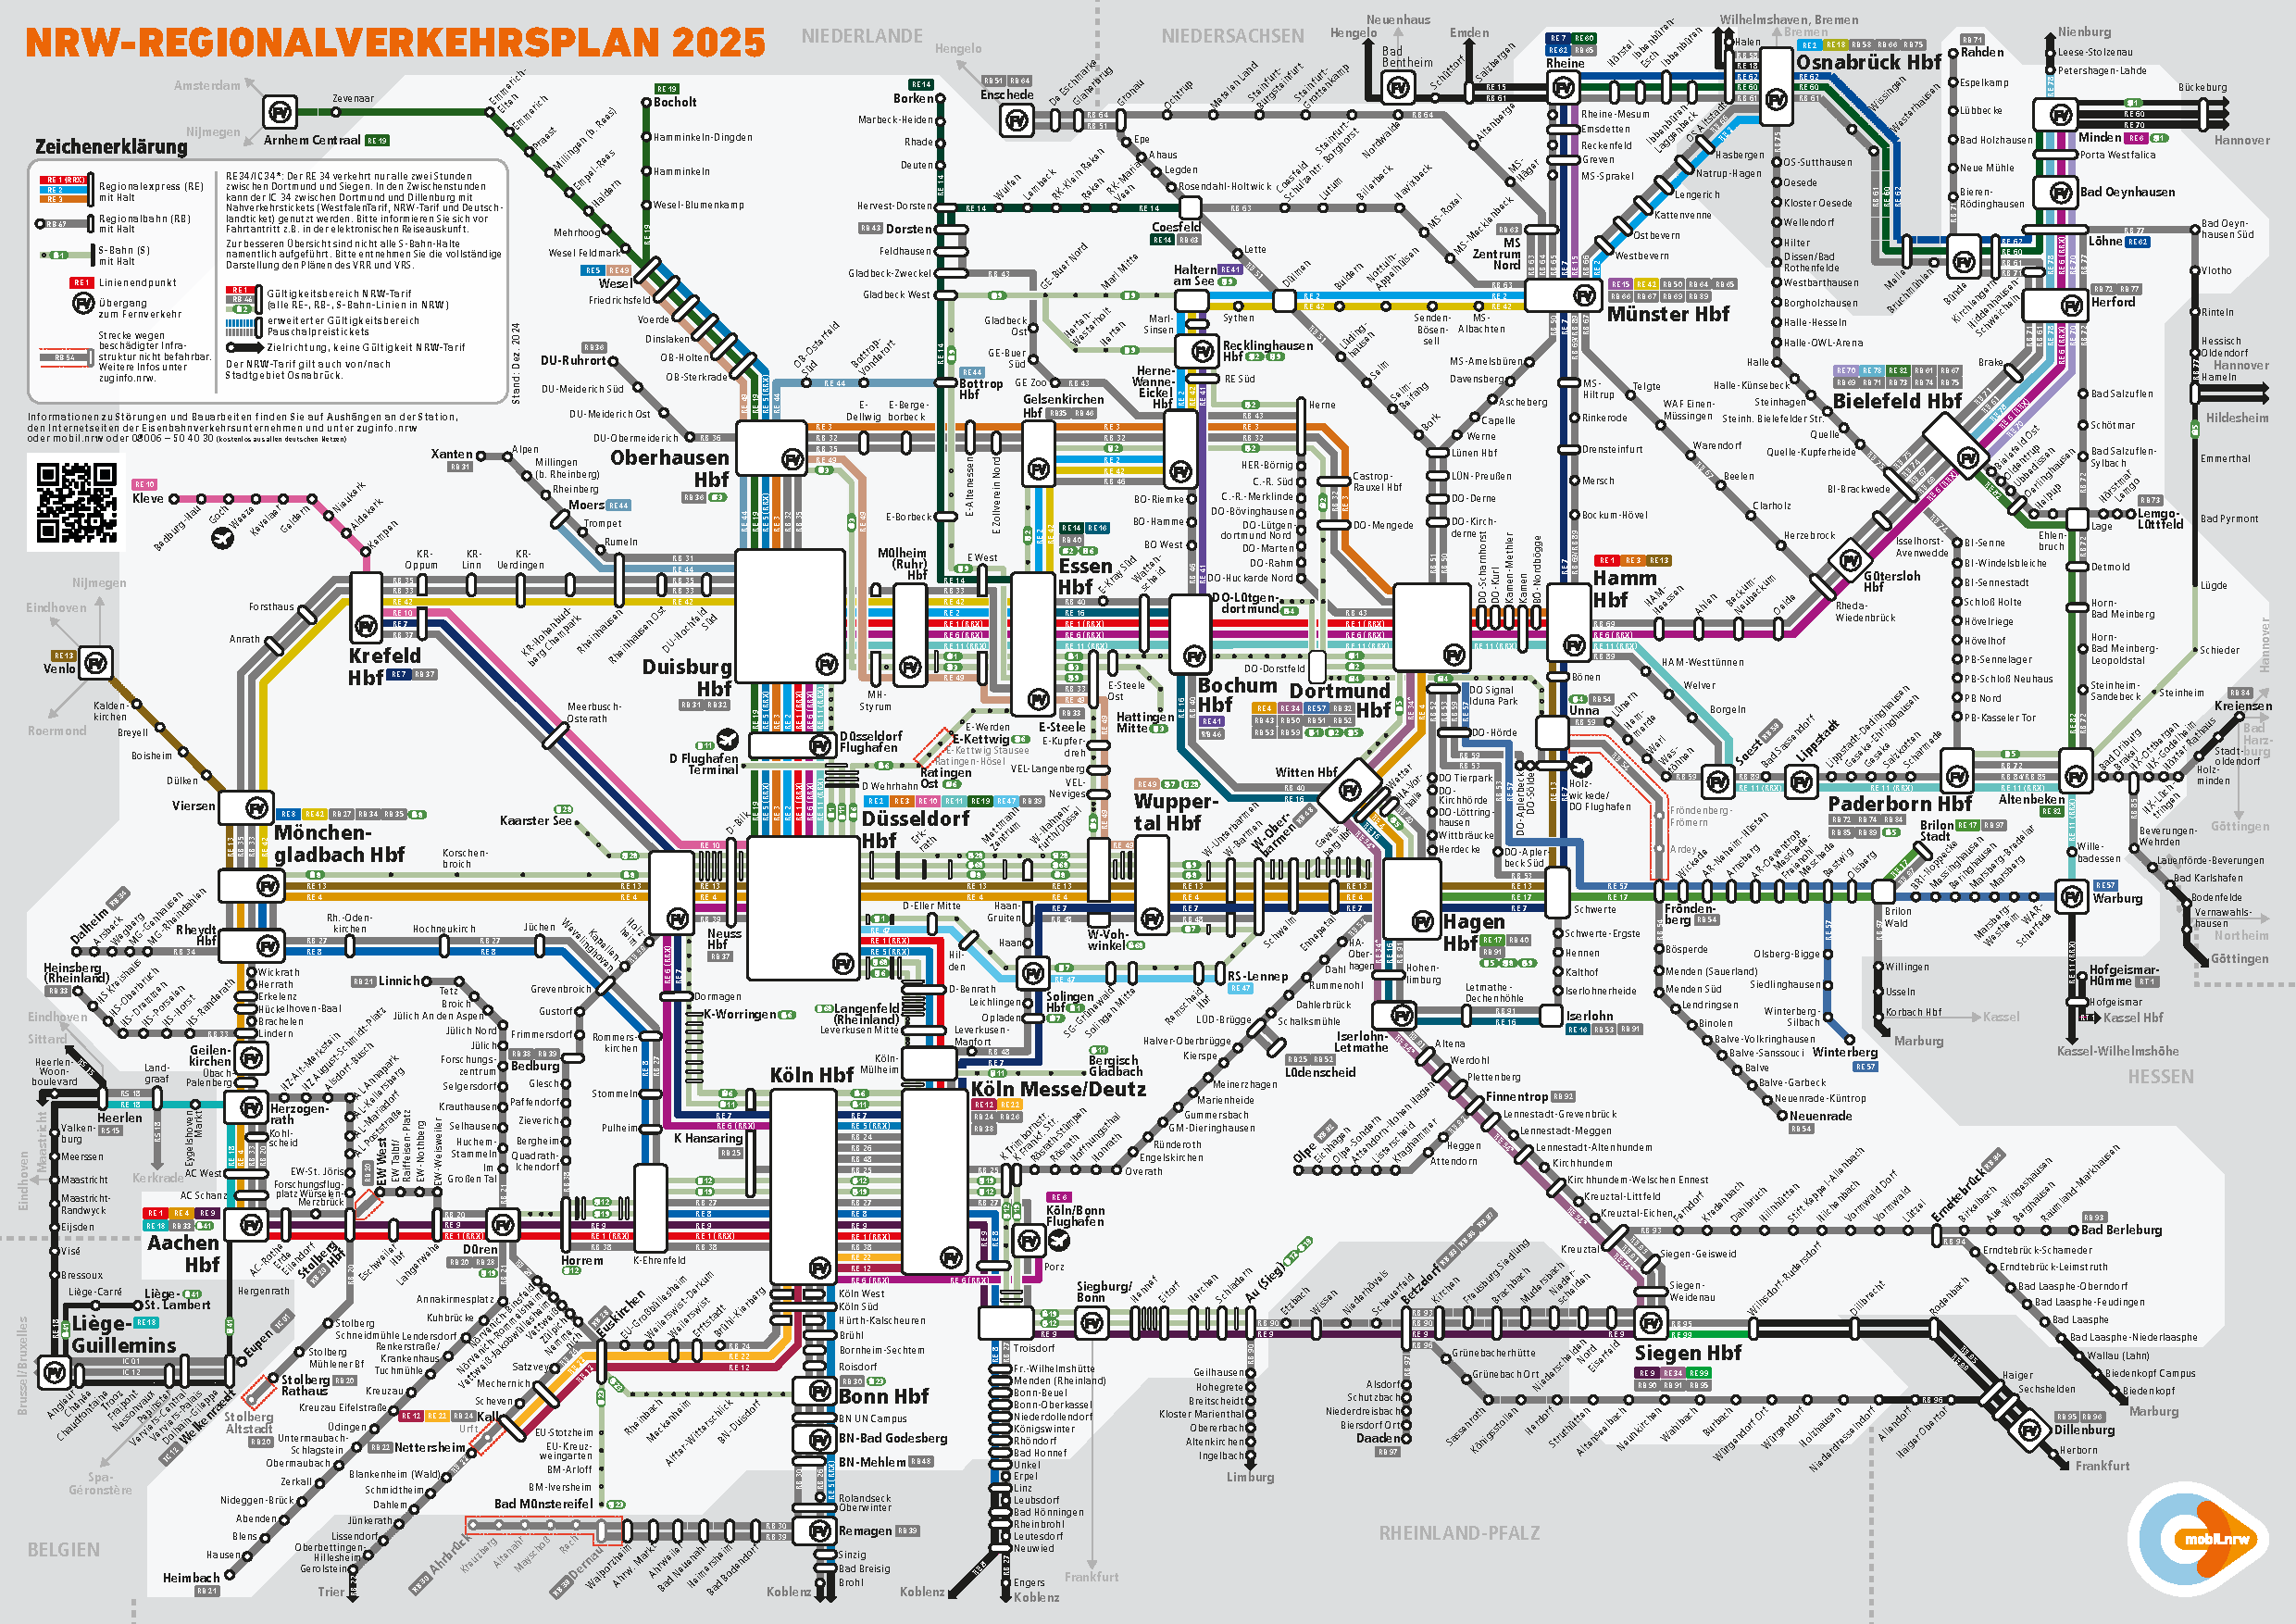
\includegraphics[width=\textwidth]{res/NRW_Regionalverkehrsplan_2025.pdf}
\end{figure*}
\textbf{Früher hab' ich mal geglaubt, das Semesterticket sei nur für den Weg nach Hause bestimmt, aber da lag ich nicht ganz richtig: Das Semesterticket~(SeTi) kann noch viel mehr.}

\includegraphics[width=\columnwidth]{res/semesterticket.pdf}

Vor Beginn jedes neuen Semesters bekommst du eine freundliche E-Mail, in der du dazu aufgefordert wirst, dich für das kommende Semester zurückzumelden. In dieser Mail ist auch ein Link zum \href{https://zividp.uni-muenster.de/idp/profile/SAML2/POST/SSO?execution=e1s1}{SelfService}-Portal enthalten, in dem du nach Bezahlen des Semesterbeitrags dein Semesterticket als PDF herunterladen kannst. Es sei hier angemerkt, dass das auch nur in dieser PDF-Datei, also nicht ausgedruckt, gültig ist.
Und wenn, gerade in den Stadtbussen Münsters, vielleicht mal vom Kontrolleur ein Auge zugedrückt werden kann, ist das Semesterticket jedoch \textit{ohne einen gültigen Lichtbildausweis nicht gültig}.

Der Universität Münster (bzw.\ dem AStA) ist es vor einigen Jahren nach langen Diskussionen und einer Urabstimmung gelungen, mit der Deutschen Bahn einen Vertrag über ein NRW-Ticket abzuschließen und dies seit dem Sommersemester 2024 als Deutschland-Ticket auszuweiten.
Daher darfst du dich im kompletten Nahverkehr in ganz Deutschland bewegen.
Zusätzlich gilt das Ticket auch für ausgewählte Bahn-Strecken außerhalb von Deutschland, z.\,B.\ von Münster nach Enschede (Niederlande). Details siehe Webseiten im "Ersti-Überlebenszettel" bzw.\ am Artikelende.

Nahverkehr bedeutet, dass du alle Busse, Straßenbahnen, U-Bahnen, S-Bahnen sowie alle Regionalbahnen -- RegionalExpress~(RE), RegionalBahn~(RB), und alle privaten Bahnen -- benutzen darfst.
Natürlich zählt der Fernverkehr -- InterCity~(IC) und InterCityExpress~(ICE) -- nicht zum Nahverkehr.

Solltest du mal mit der Bahn unterwegs sein und dein Semesterticket liegt zu Hause, ist das zwar ärgerlich, aber kein Beinbruch.
Zunächst wirst du bei der Fahrkartenkontrolle als "Schwarzfahrer" aufgeschrieben, mit dem Vorbehalt einer \SI{60}{\euro}-Strafe.
Im Rahmen dessen bekommst du ein Schreiben mit einer Zahlungsaufforderung, welches du entweder zusammen mit deinem Semesterticket am Schalter in Münster vorzeigen oder als eingescanntes Dokument zusammen mit einem Lichtbildausweis von dir an eine entsprechende Mailadresse eines Service-Centers des Zug- oder Busbetreibers senden kannst.  
Letztendlich musst du danach nur eine Bearbeitungsgebühr in Höhe von ungefähr \SI{7}{\euro} bezahlen. Ärgerlich, aber besser, als die ganzen \SI{60}{\euro} zu zahlen.

Es ist von Zeit zu Zeit ganz ratsam, sich über die Optionen deines Semestertickets neu zu informieren.
So hat zum Beispiel lange Zeit das Semesterticket dir erlaubt, in Bussen und ausgewählten Bahnverbindungen \emph{im Münsterland und Ruhr-Lippe} ab 19~Uhr sowie an Wochenenden und Feiertagen ganztägig eine weitere Person oder ein Fahrrad und bis zu drei Kinder mitzunehmen. Aufgrund des begrenzten Platzangebots ging das mit dem Fahrrad nur bei freien Stellflächen.
Da seit dem Sommersemester 2024 wie erwähnt das Semesterticket gleichbedeutend mit dem Deutschland-Ticket ist (nur als (Groß-)Teil des Semesterbeitrages vergünstigt), ist damit allerdings auch als unerwünschter Nebeneffekt die Mitnahmeregelung von eben erwähnten Fahrrädern und Personen entfallen (was nicht zwangsläufig jedem Studierenden gefallen muss). 


\subsection{Das Kultursemesterticket}
Seit es 2015 durch eine Urabstimmung in der Studierendenschaft eingeführt wurde, gibt es neben dem Semesterticket das sogenannte Kultursemesterticket. Dieses wird ähnlich wie das Semesterticket aus den Semesterbeiträgen finanziert und erlaubt Studierenden, viele kulturelle Einrichtungen in Münster vergünstigt oder sogar kostenlos zu besuchen. Dies handelt der AStA jeweils direkt mit der ensprechenden Einrichtung aus – der Grad der Vergünstigung kann daher stark variieren. So bieten z.\,B. das Stadtmuseum Münster und der Literaturverein freien Eintritt, während das Theater Münster ein festes Kontingent an Freikarten und kostenlose Restplätze anbietet. Sportfans dürfte interessieren, dass es für Fußball, Volleyball und Basketball der heimischen Teams Freikartenkontingente gibt. Wie ihr an die Tickets kommt und eine vollständige Übersicht aller aktuellen Angebote des Kultursemestertickets gibt es unter \url{https://www.asta.ms/kuseti}. 

\smallskip

\begin{center}
	%\includegraphics[width=0.25\columnwidth]{res/bushaltestelle.pdf}
	{\bfseries
	Aktualisierte Infos zum SeTi gibt es unter\\
	\url{https://www.asta.ms/semesterticket}}
	
	(weitere Links findet ihr im "Ersti-Überlebenszettel" auf Seite~\pageref{dpü} dieser Ersti-$\Phi$bel)
\end{center}

\fibelsig{Andreas G., Simon, Moritz, Marius}
\end{multicols*}



